
\begin{table*}[!t]
\renewcommand{\arraystretch}{1.3}
\caption {Prediction Accuracy for Interference Among Different Jobs Starting at Different Times}
\label{table_differentjob_differentstarttime}
\centering
\begin{tabular}{c|c|c|c|c}
\hline

\bfseries Run & \bfseries JobName & \bfseries Starting Time(s) & \bfseries First Stage & \bfseries Whole Job\\
\hline\hline
Scenario - I & PR & 0 & 0.91 & 0.81\\
& KM & 38 & 0.99 & 0.94\\
& LR & 26 & 0.94 & 0.94 \\
& WC & 78 & 0.83 & 0.82\\
\hline
Scenario - II & PR & 91 & 0.90 & 0.82\\
& KM & 0 & 0.79 & 0.77\\
& LR & 48 & 0.87 & 0.88\\
& WC & 53 & 0.99 & 0.93\\
\hline
Scenario - III & PR & 20 & 0.99 & 0.90\\
& KM & 87 & 0.98 & 0.91\\
& LR & 0 & 0.84 & 0.85\\
& WC & 48 & 0.98 & 0.91\\
\hline
Scenario - IV & PR & 77 & 0.93 & 0.85\\
& KM & 25 & 0.72 & 0.71\\
& LR & 86 & 0.99 & 0.99 \\
& WC & 0 & 0.99 & 0.93\\
\hline
\end{tabular}
\end{table*} 



% Run B

\begin{table*}[!htb]
\renewcommand{\arraystretch}{1.3}
\caption{Execution Time Prediction for PageRank Job in Scenario - I}
\label{bpr}
\centering
\begin{tabular}{l|r|r|r|r|r|r}
\hline
\bfseries StageNo & \bfseries 1 & \bfseries 2 & \bfseries 3 & \bfseries 4 & \bfseries 5 & \bfseries 6 \\
\hline \hline
Actual Time (s)
&575.3
&36.4
&33.7
&24.1
&22.5
&55.8 \\
\hline
Predicted Time (s) 
&522.9
&43.0
&10.6
&5.4
&5.0
&28.3 \\
\hline
\end{tabular}
\end{table*}

\begin{table*}[!htb]
\renewcommand{\arraystretch}{1.3}
\caption{Execution Time Prediction for K-Means Job in Scenario - I}
\label{bkm}
\centering
\begin{tabular}{l|r|r|r|r|r|r|r|r|r|r|r|r}
\hline
\bfseries StageNo & \bfseries 1 & \bfseries 2 & \bfseries 3 & \bfseries 4 & \bfseries 5 & \bfseries 6 & \bfseries 7 & \bfseries 8 & \bfseries 9 & \bfseries 10 & \bfseries 11 & \bfseries 12\\
\hline \hline
Actual Time (s)
&611.8
&6.9
&21.0
&8.2
&18.0
&7.5
&17.6
&7.2
&17.5
&7.1
&17.3
&6.9 \\
\hline
Predicted Time (s) 
&610.7
&7.4
&25.2
&18.1
&22.9
&9.7
&23.6
&8.4
&23.2
&9.2
&24.8
&6.2 \\
\hline
\end{tabular}
\end{table*}

\begin{table*}[!htb]
\renewcommand{\arraystretch}{1.3}
\caption{Execution Time Prediction for Logistic Regression Job in Scenario - I}
\label{blr}
\centering
\begin{tabular}{l|r|r|r|r|r|r|r|r|r|r}
\hline
\bfseries StageNo & \bfseries 1 & \bfseries 2 & \bfseries 3 & \bfseries 4 & \bfseries 5 & \bfseries 6 & \bfseries 7 & \bfseries 8 & \bfseries 9 & \bfseries 10 \\
\hline \hline
Actual Time (s)
&576.8
&7.4
&7.3
&7.4
&7.2
&7.1
&7.8
&7.3
&7.2
&7.1 \\
\hline
Predicted Time (s) 
&617.1
&7.1
&7.2
&7.6
&6.6
&7.0
&6.5
&7.9
&6.9
&6.3
\\
\hline
\end{tabular}
\end{table*}


\begin{table*}[!htb]
\renewcommand{\arraystretch}{1.3}
\caption{Execution Time Prediction for WordCount Job in Scenario - I}
\label{bwc}
\centering
\begin{tabular}{l|r|r}
\hline
\bfseries StageNo & \bfseries 1 & \bfseries 2 \\
\hline \hline
Actual Time (s)
& 615.2
& 61.8 \\
\hline
Predicted Time (s) 
& 506.5
& 77.8 \\
\hline
\end{tabular}
\end{table*}


\nop{maifi

\begin{figure}[!t]
\centering
\captionsetup{justification=centering}
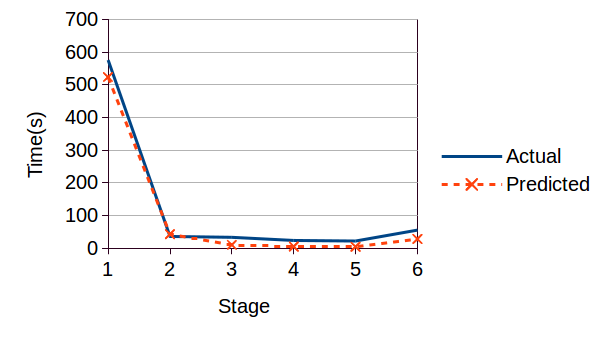
\includegraphics[width=3in]{B_pr.png}
\caption{Execution Time Prediction for PageRank Job in Scenario - I}
\label{bpr}
\end{figure}

\begin{figure}[!t]
\centering
\captionsetup{justification=centering}
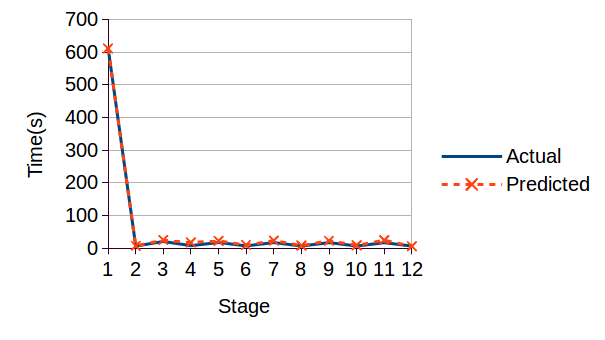
\includegraphics[width=3in]{B_km.png}
\caption{Execution Time Prediction for K-Means Job in Scenario - I}
\label{bkm}
\end{figure}

\begin{figure}[!t]
\centering
\captionsetup{justification=centering}
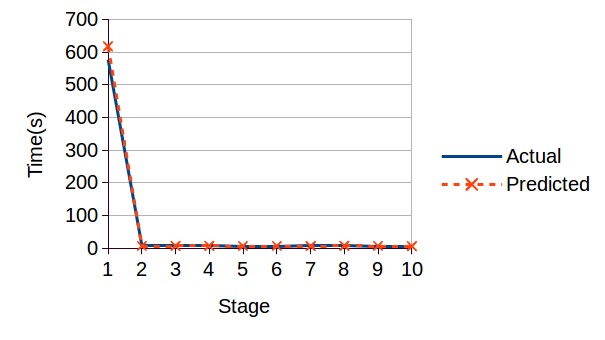
\includegraphics[width=3in]{B_lr.png}
\caption{Execution Time Prediction for Logistic Regression Job in Scenario - I}
\label{blr}
\end{figure}

\begin{figure}[!t]
\centering
\captionsetup{justification=centering}
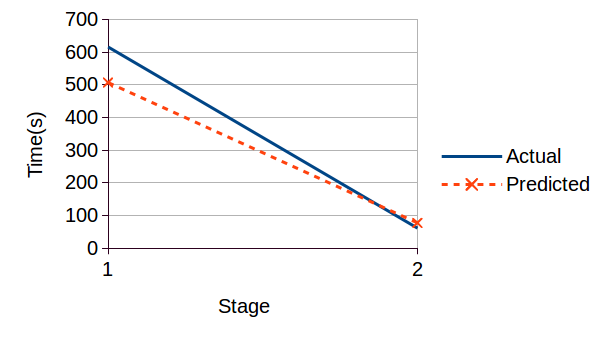
\includegraphics[width=3in]{B_wc.png}
\caption{Execution Time Prediction for WordCount Job in Scenario - I}
\label{bwc}
\end{figure}

}


\subsection{Interference Among Multiple Jobs Starting at Different Times}
\label{newsection}
Finally, to test the prediction accuracy of our model where different jobs may arrive and start at different times, we use the four Apache Spark jobs and input data set as before, and start them randomly at different times. To ensure that each job will interfere with at least one other job while executing, we set the starting time for each job as $startingTime \in [minstagetime / 10, \\
minstagetime / 2]$, where $minstagetime$ represents the smallest execution time for the first stage among all the jobs. In our case, $minstagetime=190 sec$, causing the starting time for different jobs to be between 19 sec and 95 sec.

\noindent
Given the above range, for evaluation, we randomly pick one job and start at time 0, and then 
set the starting time for the remaining three jobs between 19 sec and 95 sec randomly. 
We considered four scenarios where the starting job is different in each scenario. The prediction accuracy for the whole job while running four different jobs in parallel starting at different times is summarized in Table~\ref{table_differentjob_differentstarttime}. As shown in the table, in our evaluation, prediction accuracy ranges between 99\% and 71\% for the whole job, and between 99\% and 72\% for the first stage. The predicted execution time and the actual execution time for PageRank, K-Means, Logistic Regression, and WordCount under Scenario - I are shown in Table~\ref{bpr}, Table~\ref{bkm}, Table~\ref{blr}, and Table~\ref{bwc} respectively. 



